% Figure 1 (full width). Generated by make_figures.py (fig1).
\begin{figure*}[t]
  \centering
  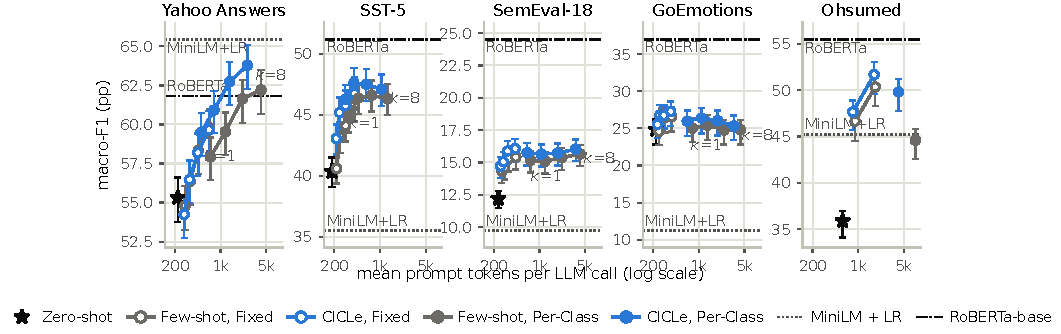
\includegraphics[width=\textwidth]{figures/f1_vs_tokens.pdf}
  \caption{Macro-F1 against mean prompt tokens per LLM call (log scale), one panel per dataset. Every point is one (method, retrieval variant, $k$) at the reference setting, averaged over six models and three seeds, with $k$ increasing along each line. Hollow markers: Fixed retrieval. Filled: Per-Class. Grey: few-shot. Blue: CICLe. Star: zero-shot. Dotted and dash-dot lines: MiniLM with logistic regression and fine-tuned RoBERTa-base (three-seed means). Error bars are 95\% bootstrap intervals of the 18-run mean over test instances, not the spread over hyperparameters. Ohsumed Per-Class is $k = 1$ only.}
  \label{fig:tokens}
\end{figure*}
